\chapter{Literatuurstudie}
\label{Literatuurstudie}
Dit hoofdstuk verduidelijkt de theorie en de kennis die nodig is om het onderzoek in deze masterproef te begrijpen. Als eerste bespreken we de werking van satellieten in sectie \ref{LSat}. Vervolgens wordt er een beeld van de satelliet constellaties die gebruikt worden geschetst. Deze worden besproken in sectie \ref{LGNS}. Eens we de verschillende types van satellieten kennen, wordt in sectie \ref{LEPN} het Europees permanent netwerk besproken. De verschillende soorten communicate worden besproken in sectie \ref{LCom}.

\section{Satellieten}
\label{LSat}
Om de werking van de satelliet systemen beter te begrijpen, verklaren we in deze sectie eerst een paar basis principes. In sectie \ref{LPbS} verklaren we hoe aan de hand van satellieten de positie bepaald kan worden. Vervolgens bespreken we de verschillende types van satellieten  besproken in sectie \ref{LVTS}. Satellieten worden geobserveerd en gestuurd door grondstations. Die zorgen voor de ruimtelijke informatie in het signaal. Dit is de ephemeris data (de baan van een satelliet) of de almanak data (de realtie tussen alle satellieten). Bijkomend wordt informatie over de klok verzonden \cite{LBibGNSS8}.

\subsection{Positie bepaling aan de hand van satellieten}
\label{LPbS}
Het algemeen principe achter een satelliet navigatie systeem is de trilateratie vanuit elk punt op het oppervlak van de aarde ten op zichte van de zichtbare satellieten.  De afstand tot de satellieten wordt gemeten door de tijd die het radiosignaal nodig heeft om de ontvanger te bereiken. Omdat het radiosignaal reist aan de lichtsnelheid, worden zeer nauwkeurige klokken gebruikt. De satellieten bevatten atomaire klokken, de ontvangers geavanceerde quartz klokken. De exacte locatie van de satelliet wordt bekeken als een gekende voor de rest van de positiebepaling. Dit is mogelijk omdat de banen van de satellieten zeer stabiel en voorspelbaar zijn. In principe zijn drie satellieten voldoende om een drie dimensionale positie te bepalen. Alle punten met de zelfde afstand tot een satelliet vormen een sferisch oppervlak met de satelliet in het midden. Drie sferische oppervlakken snijden elkaar in twee punten. E\'en van deze punten kan verwaarloosd worden omdat de positie te ver is van het aardoppervlak. Dit is grafisch weergegeven in figuur \ref{imgPbS} Een vierde signaal is nodig om de tijdsverschillen te elimineren tussen de klokken van de satellieten en de ontvanger. Het aantal ontvangers is niet gelimiteerd omdat gebruikers zich op een passieve manier gedragen.
 
\begin{figure}[hbp]
	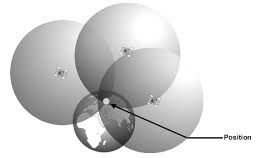
\includegraphics[scale=1.65]{BepalingPositie.jpg}
	\centering
	\caption{Positie bepaling aan de hand van satellieten \cite{LBibSat}}
	\label{imgPbS}
\end{figure} 

De berekende positie heeft een foutenmarge in de grote orde van enkele meters . Dit is echter voor veel toepassingen, zoals de navigatie in de auto voldoende nauwkeurig). De grootste oorzaken van fouten zijn de volgende \cite{LBibGNSS8}:
\begin{itemize}
	\item De geometrische positie van de satellieten, bij elke satelliet kan er een kleine afwijking zijn ten op zichte van de postie die men als gekend rekent
	\item Klok fouten zowel bij de satelliet als de ontvanger
	\item Troposferische en ionosferische condities
	\item Multipad effecten
	\item Onjuistheden van de ontvanger
\end{itemize}

\subsection{Verschillende types satellieten}
\label{LVTS}
Satellieten worden onderverdeeld in verschillende types. Dit heeft voornamelijk te maken met de baan die ze hebben rond de aarde en hun positie ten opzichte van een punt op het aardoppervlak. In deze sectie worden twee verschillende soorten van satellieten besproken. 

\subsubsection{Geostationary Earth Orbit Satelliet}
Geostationary Orbit satelliet. Dit wordt vaak afgekort als GEO \cite{LBibGEO,LBibMEO}. Het gebied waarin GEO satellieten voorkomen is net zoals Low Earth Orbit (LEO) gebied beschermd \cite{LBibMEO}. De GEO satellieten hebben per definitie dezelfde omwentelingsnelheid rond de aarde als dat de aarde om haar as draait. Hierdoor lijken zij bekeken vanuit een punt op de aarde stationair \cite{LBibGEO}.  Vaak is de nauwkeurigheid van de satellietbaan van een GEO satelliet minder nauwkeurig dan deze van een ander satelliet type. Dit kan verklaart worden door het feit dat er geen geometrische variatie is tussen de GEO satelliet en het referentiestation. Hiermee bedoelt men dat de positie van de satelliet tegen over het referentie station op aarde gelijk blijft. Indien de satelliet afwijkt van zijn baan, wordt dit wel gemten, maar zou dit ook door een andere fout zoals bijvoorbeeld een klok fout kunnen komen. Hierdoor wordt de afwijking in de satelliet baan pas laat gedetecteerd. Dit verzwakt de schatting van de satellietbaan \cite{LBibPPP2}. 
 
\subsubsection{Medium Earth Orbit satelliet}
Medium Earth Orbit (of afgekort MEO) satellieten bewegen als je kijkt vanop de aarde \cite{LBibGEO}. MEO is geen beschermd gebied. MEO wordt gedefinieerd als een regime van satellietbanen met hoogtes tusen LEO en de geosynchrone riem. Dit betekent dat de hoogtes zich bevinden tussen 2000 km en 35586 km.  GNSS (wordt verder besproken in sectie \ref{LGNS}) constellaties zijn gelocaliseerd in grote MEO hoogtes tussen 18 000 km en 24 000 km. Met constellaties worden netwerken van satellieten bedoeld. Kleine MEO hoogtes tot 5000 km kunnnen interessant zijn voor kleine satelliet missies. 85\% Van de satellieten in het MEO gebeid maken deel uit van 6 groepen \cite{LBibMEO}:

\begin{enumerate}
	\item GLONASS: Verder besproken in sectie \ref{LGLO}. 
	\item NavStar: De GPS satellieten, deze worden uitgebreid besproken in sectie \ref{LGPS}
	\item Initial Defence Satellite Communications System. De voorganger van het Amerikaans Defentie Satelliet Communicatie Systeem. De satellieten werden gelanceerd in 1960 in circulaire banen in het MEO gebied
	\item  Oko: Dit is de Russiche defentie constellatie. De satellieten zijn geplaatst in een Molniya satellietbaan. Molniya satllietbanen zijn banen met een eliptische vorm,  waar de aarde niet het middelpunt is. De banen zijn geplaatst in een hoek van 63.4 graden ten op zichte van de evenaar
	\item Nieuwe GNSS constellaties: Galileo, meer informaite hierover is te vinden in sectie \ref{LGal} en BeiDou, besproken in sectie \ref{LBeD}
	\item West Ford needle experiment: dit is technisch gezien geen constellatie. De naalden zijn in 1960 gelanceerd om de lange afstand HF communicatie te verbeteren. 
\end{enumerate}
Er was veel intresse in MEO eind 1960. Maar sindsdien is er niet veel gebeurt tot 1980. De satelliet navigatie constellaties omvatten het grootste deel van MEO lanceringen in de laatste dertig jaar \cite{LBibMEO}.

\section{Global Navigation Satellite System}
\label{LGNS}
GNSS ofwel Global Navigation Satellite System, is een satelliet systeem met een wereldwijde dekking van het aardoppervlak. GNSS is een standaard term, gebruikt om systemen te beschrijven die positie en navigatie oplossingen bieden. Het werd voornamelijk ontwikkeld voor de luchtvaart en ruimtevaart industrie en voor militaire doeleinden. Tegenwoordig worden deze technologie\"en ook in andere toepassingen gebruikt, zoals in de wetenschap om de beweging van de continenten te bestuderen of landmeters die aan de hand van satellieten metingen doen. GNSS vraagt samenwerking tussen verschillende publieke en private organisaties \cite{LBibGNSS3}. GNSS satellieten zenden continu radiosignalen uit naar de oppervlakte van de aarde door de atmosfeer \cite{LBibGPS4}. Het GNSS systeem is opgebouwd uit verschillende constellaties die verder in deze tekst besproken worden. GPS, besproken in sectie \ref{LGPS}, is de eerste constellatie van GNSS. In sectie \ref{LGLO} bespreken we GLONASS, dit zijn beide militaire systemen. Toch zijn ze beschikbaar voor gebruik door internationale private en commerci\"ele doeleinden \cite{LBibGNSS8}. Galileo wordt besproken in sectie \ref{LGal} en BeiDou komt al laatste aan bod in sectie \ref{LBeD}. GNSS bestaat momenteel uit zes constellaties. Het Quasi-Zenith Satellite System (Japan) en Indian Redional Navigation Satellite System worden niet besproken. Doordat BeiDou en Galileo relatief nieuwe systemen zijn, hebben zij qua modellering beperkingen tegenover de oudere systemen, zoals GPS en GLONASS. De precise antenne fase verbeteringen zijn beschikbaar voor GPS en GLONASS. Voor Galileo en BeiDou zijn deze momenteel nog niet beschikbaar \cite{LBibPPP2}. De GNSS constellaties zijn opgebouwd uit drie delen, namelijk het ruimte gedeelte, het controle gedeelte en het gebruikers gedeelte \cite{LBibBeiDou2}.  Het IGS, International GNSS Service staat in voor de aflevering van de hoogste kwaltieit GNSS data en producten \cite{LBibGNSS}. Het IGS geeft op regelmatige basis de meest accuratie informatie over satellietbanen en klokken voor GPS en GLONASS vrij. Dit wordt mogelijk gemaakt door een dicht globaal netwerk en verschillende meewerkende data analyse centra. Voor de schatting van satellietbanen en klokken wordt een software pakket (NAPEOS) gebruikt. De software is uitgebreid om de vier besproken constellaties te verwerken \cite{LBibPPP2}. Elke satelliet is een project op zichzelf. Hierdoor is het moeilijk om een gestandaardiseerde productie ketting te cre\"eren \cite{LBibGNSS3}. Om de performantie van GNSS te meten zijn beschikbaarheid, betrouwbaarheid en nauwkeurigheid sleutelparameters. Met de beschikbaarheid bedoelt men het aantal satellieten dat zichtbaar is vanaf de positie van de gebruiker.De nauwkeurigheid is een maat voor hoe groot her verschil is tussen de werkelijke en de berekende postie en snelheid \cite{LBibGNSS6}. De nodige nauwkeurigheid is afhankelijk van de toepassing waarin het gebruikt wordt \cite{LBibRTK3}. Gebruikers merkten al in het begin op dat de satellieten van een constellatie in het zelfde gedeelde van de hemel voorkomen met een periode die net iets kleiner is dan \'e\'en dag. Dit was een belangrijke eigenschap toen het systeem nog niet volledig was en data verzameld moest worden op het moment dat de meeste satellieten zichtbaar waren \cite{LBibGNSS7}. Dit komt doordat voor nauwkeurige metingen te hebben er vijf satellieten zichtbaar moeten zijn. In de begin jaren, waren er nog niet veel satellieten en kon men aan de hand van de periode op voorhand bepalen wanneer de meeste satellieten zichtbaar zijn op het punt waar de metingen moeten gebeuren. Zodat ze zeker voldoende zichtbare satellieten zouden hebben op het meet moment. Ondertussen is het systeem onmisbaar en komen er steeds meer extra toepassingen bij \cite{LBibGNSS8}.

\subsection{Global Postioning System}
\label{LGPS} 
Global Positioning System, wordt vaak afgekort naar GPS. Dit is het op satellieten gebaseerde positie systeem dat bij ons het bekendste is. Het is ontwikkeld in Amerika \cite{LBibGNSS, LBibGNSS3}. Het GPS systeem heeft zijn werkende capaciteit (FOC = Fully Operational Capability) bereikt in 1993 \cite{LBibGPS4}. Het is \'e\'en van de langst en meest gebruikte systemen binnen GNSS en draait momenteel op volledige capaciteit \cite{LBibGNSS4,LBibGNSS8}. GPS wordt vaak gebruikt als algemene term voor satelliet navigatie. Het primair doel van GPS is drie dimensionale navigatie \cite{LBibGNSS8}.Hiervoor maakt het gebruik van een netwerk van dubbele frequentie GPS ontvangers \cite{LBibGPS5}. Voor de gebruikers is kost van de data een hoge bezorgdheid. Daarom is het belangrijk om de kosten van de operaties te verkleinen. GPS moet toegankelijk zijn voor meerdere clients op het zelfde moment. De gebruikerstoegang gebeurt voornamelijk door mobiele toestellen die verbindig maken via het internet \cite{LBibGPS}. Voor sommige toepassingen voldoet de nauwkeurigheid en de betrouwbaarheid van de GPS constellatie niet \cite{LBibGNSS6}.

\subsubsection{Opbouw GPS constellatie}
 De constellatie van GPS bestaat uit 32 satellieten en heeft zijn FOC bereikt, het systeem wordt geleidelijk aan gemoderniseerd \cite{LBibGNSS4}. De satellieten zijn geplaatst in een bijna circulaire baan met een straal van 2562.75km. De periode bedraagt 11 uur en 58 minuten \cite{LBibGNSS6,LBibGNSS8}. Dit is de tijd die verstrijkt tussen dat een satelliet terug op dezelfde plaats wordt waargenomen. De satellieten werden geplaatst in zes orbitale vlakken. De satellieten in elk vlak zijn niet op gelijke afstand geplaatst \cite{LBibGNSS6}. Deze constellatie voorziet de gebruiker van vijf tot acht zichtbare satellieten vanop elk punt op het aardoppervlak \cite{LBibGNSS8}. De opbouw van de constellatie wordt grafisch weergegeven in figuur \ref{imgGPS}.
 
 \begin{figure}[hbp]
 	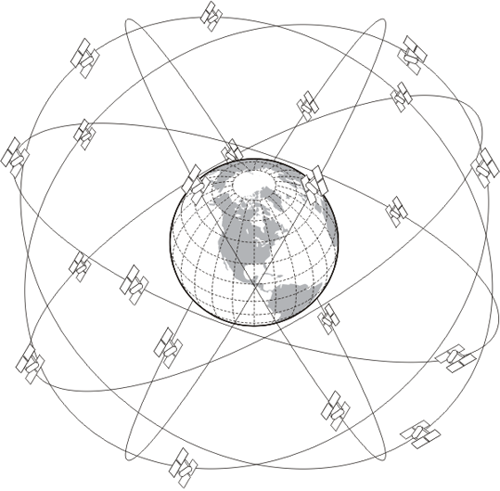
\includegraphics[scale=0.95]{GPS.png}
 	\centering
 	\caption{GPS constellatie \cite{LImgGPS}}
 	\label{imgGPS}
 \end{figure}

\subsubsection{ GPS Signalen}
Het GPS signaal bestaat uit twee zeer stabiele, bijna monochromatische draaggolven L1 en L2, waarop drie modulaties op aanwezig zijn \cite{LBibBeiDou4}:
\begin{itemize}
	\item C/A code
	\item P code
	\item broadcast bericht
\end{itemize}
Alle componenten van een GPS signaal zijn gebaseerd op een fundamentele kloksnelheid (f\textsubscript{0}) van 10,23 MHz. De GPS draaggolven hebben een frequentie van 154 f\textsubscript{0} voor L1 en een frequentie van 120 f\textsubscript{0} voor L2\cite{LBibGPS2}. De nauwkeurigheid van L1 code en de metingen van de fase van de draaggolf (CP) zijn nauwkeuriger dan deze bij L2 \cite{LBibBeiDou4}. GPS signalen zijn modulaties van de draaggolven L1 en L2 van alle satellieten \cite{LBibGPS3}. Er is ook een nieuwer signaal is L5, dit wordt uitgestraald door de nieuwste generatie van GPS satellieten. L5 wordt gebruikt voor Safety of Life toepassingen. Het wordt uitgestraald met een frequentie gelijk aan f\textsubscript{0}. Dit signaal wordt slechts door een beperkt aantal ruimtetuigen gebruikt \cite{LBibGNSS9}.

\subsubsection{Manieren om posities te bepalen}
Er zijn verschillende technieken om uw positie te bepalen. Deze kunnen verschillen in het aantal stations dat nodig is. Verder wordt er voor sommige toepassingen aan post-processing gedaan, terwijl andere toepassingen een real-time aanpak vragen. De verschillende methodes verschillen ook in de te behalen nauwkeurigheid. In deze tekst worden drie verschillende methodes besproken. 

\paragraph{Differential GPS Corrections}
Differential GPS Corrections, ook wel DGPS genoemd, worden gebruikt om nauwkeurig posities  te bepalen \cite{LBibGLONASS2}. Dezelfde techniek wordt ook gebruikt op GNSS niveau, men spreekt dan van DGNSS \cite{LBibGNSS8}. Er worden minimaal twee GPS ontvangers gebruikt. Voor \'e\'en van deze ontvangers moet de precise postie gekend zijn, dit noemen we de basis ontvanger \cite{LBibGNSS2,LBibRTK}. De twee stations moeten zich dicht bij elkaar bevinden (afstand kleiner dan 10 km) \cite{LBibDGPS}. De basis ontvanger gaat data (bv zijn postitie bepaald aan de hand van satellieten) verzenden over een radio link naar het tweede station.  Dit tweede station kan in beweging zijn, dit is echter geen voorwaarde. Het tweede station berekent zijn positie aan de hand van de data die hij ontvangt van de satellieten, maar ook van de data die hij krijgt via de radio link van het basis station \cite{LBibRTK}. Dit is een veel gebruikte manier om satelliet- en klokfouten te elimineren. Een nadeel van deze techniek is dat de observaties van beide stations simultaan moeten gebeuren \cite{LBibGNSS2}. Deze techniek geeft meestal een resultaat op 1m nauwkeurig \cite{LBibRTK}. Deze metingen gebeuren aan de hand van de pseudo range data. Ze worden niet real-time gemaakt \cite{LBibRTK3}.

\paragraph{Real-Time Kinematic}
Real-Time Kinematic wordt afgekort als RTK. RTK is een speciale vorm van DGPS dat ongeveer centimeter nauwkerigheid aanbiedt. Indien je, door gebruik te maken van dit algoritme, de positie wilt bepalen, moeten er minimaal vijf satellieten zichtbaar zijn. Anders werkt het niet, of even traag als DGPS in vele toepassingen \cite{LBibRTK}. Bij RTK wordt de positie berekend door te werken met de CP dit is de fase van de draaggolf \cite{LBibRTK2}. De CP is de meer nauwkeurige versie van de pseudo range. De draaggolf heeft normaal een constante frequentie. Maar de ontvangen draaggolf heeft een veranderende frequentie door de beweging van de satelliet en de ontvanger, er gaat een Doppler effect optreden. Voor nauwkeurige positie bepaling worden de metingen die door \'e\'en ontvanger gemaakt worden gecombineerd met de metingen van een tweede ontvanger die simultaan gemaakt worden \cite{LBibRTK3}. Het referentie station of ook wel het basis station genoemd, gaat de CP en de pseudo range metingen van de zichtbare satellieten bepalen. Deze worden via een datalink naar de andere stations gestuurd \cite{LBibDGPS}. Deze werking wordt verduidelijkt in figuur \ref{imgRTK}. 

\begin{figure}[h!bp]
	\includegraphics[scale=0.5]{RTK.jpg}
	\centering
	\caption{Schematische weergave van een RTK systeem \cite{LBibDGPS}}
	\label{imgRTK}
\end{figure}

In een RTK systeem gaan zowel het basis station en het bewegende station bestaan uit een single -of dual GPS ontvanger, de geassocieerde antenne en een data radio. Typisch gebruiken gebruikers identieke GPS ontvangers en data radios bij beide stations \cite{LBibRTK3}. RTCM berichten (dit wordt verder besproken in secte \ref{LRTC}) 18 tot 21 bevatten de meeste data die nodig zijn voor een succesvol RTK systeem \cite{LBibDGPS} .


\paragraph{Precise Point Positioning}
Precise Point Postioning of PPP is een techniek die werkt met \'e\'en ontvanger en is zeer effici\"ent. \cite{LBibGNSS4}. De PPP techniek wordt steeds belangrijker in hoge precisie positie toepassingen \cite{LBibPPP2}. PPP is momenteel gebaseerd op enkel GPS observaties. De nauwkeurigheid, beschikbaarheid en bertrouwbaarheid zijn sterk afhankelijk van het aantal zichtbare satellieten. Deze is vaak onvoldoende op bepaalde plaatsen. De nauwkeurigheid en de bertrouwbaarheid kan be\"invloed worden door slechte satelliet geometrie. Een mogelijke manier om de beschikbaarheid van satellieten te doen stijgen is om GPS en GLONASS resultaten te integreren. Daar wordt momenteel veel onderzoek naar gedaan \cite{LBibPPP}. In post-processing kan centimeter level nauwkeurigheid bereikt worden. Voor kinematische toepassingen wordt decimeter level nauwkeurigheid bereikt \cite{LBibGPS2}.  

\subsection{GLONASS}
\label{LGLO}
GLONASS is \'e\'en van de langst gebruikte systemen binnen GNSS. Het is ontwikkeld door Rusland \cite{LBibGLONASS2}. GLONASS is een afkorting, het staat voor GLObal'naya NAvigatsionnaya Sputnikovaya Sistema of in het Engels: GLObal NAvigation Satelite System  \cite{LBibBeiDou,LBibGNSS8}. GLONASS heeft veel gemeenschappelijk met GPS, met name de opbouw van de constellatie, de banen van de satellieten en signaal structuur. E\'en van de grootste verschillen tussen GLONASS en GPS is het referentie systeem waarin de co\"ordinaten geleverd worden \cite{LBibGNSS8}.Het GLONASS systeem is opgebouwd uit vier elementen \cite{LBibGLONASS2}:
\begin{itemize}
	\item constellatie van GLONASS satellieten
	\item Controle segment op de grond
	\item Rakket/ruimte complex
	\item Gebruikers
\end{itemize} 
Het systeem wordt continu gemoderniseert \cite{LBibGNSS4}. GLONASS-M satellieten vormen een tweede generatie van satellieten die gebruikt worden\cite{LBibGNSS}. De M staat voor Modified (aangepast). Deze satellieten werden in gebruik genomen in 2003 \cite{LBibPPP}. Deze tweede generatie heeft de volgende voordelen \cite{LBibGLONASS,LBibPPP}:
\begin{itemize}
	\item Langere gegarandeerde levenstijd (zeven jaar in plaats van drie)
	\item Maakt gebruik van L2 signalen
	\item Stabielere klok
	\item Extra beschikbare navigatie data (zoals betere integritetiscontrole, informatie over absolute tijd beschikbaarheid van de satelliet nummer)
	\item inter-satelliet radio link
	\item Betere zonnenpanelen positionering
	\item Lager kans op onvoorspelde versnellingen
\end{itemize}
Door deze tweede generatie GLONASS satellieten zijn er nieuwe mogelijkheden voor satelliet navigatie. GLONASS is een betrouwbaar systeem, voornamelijk voor Real-Time Kinematic (RTK) toepassingen in omgevingen met slechte zichtbaarheid \cite{LBibGLONASS}. Voor de werking van het navigatie satelliet systeem is het belangrijk dat alle processen die plaats vinden tijdens de werking gesynchroniseerd zijn. GLONASS-K satellieten vormen de derde generatie. De grootste veranderingen ten opzichte van GLONASS M zijn \cite{LBibGLONASS2}:
\begin{itemize}
	\item Het gebruik van een derde frequentie om betrouwbaarheid en nauwkeurigheid voor gebruikersnavigatie te vergroten.
	\item De levensduur van de satelliet is vergroot tot 10 jaar
	\item Het gewicht van de satelliet is gehalveerd
\end{itemize}
Deze satellieten zijn vanaf 2008 in gebruik genomen \cite{LBibPPP}.

\subsubsection{Opbouw GLONASS constellatie} 
De constellatie is opgebouwd uit 24 satellieten \cite{LBibGNSS4}. De satellieten bevinden zich op bijna circulaire banen met een straal die net iets kleiner is dan 20 000 km. Deze satellieten bevinden zich in het MEO gebied \cite{LBibMEO}. De satellieten zijn geplaatst in drie orbitale vlakken met een onderlinge afstand van 120 graden \cite{LBibGLONASS2,LBibGNSS6, LBibGNSS8}. Per vlak zijn er acht satellieten geplaatst. De periode per satelliet voor \'e\'en omwentelling rond de aarde is 11 uur en 15 minuten \cite{LBibGNSS6}.  Het systeem heeft zijn FOC bereikt in januari 1996 \cite{LBibGLONASS}. Het systeem is volledig gerevisioneerd en is volledig operationeel \cite{LBibGNSS4}. Een grafische weergave van de GLONASS constellatie is te zien in figuur \ref{imgGLONASS}.

\begin{figure}[h!]
	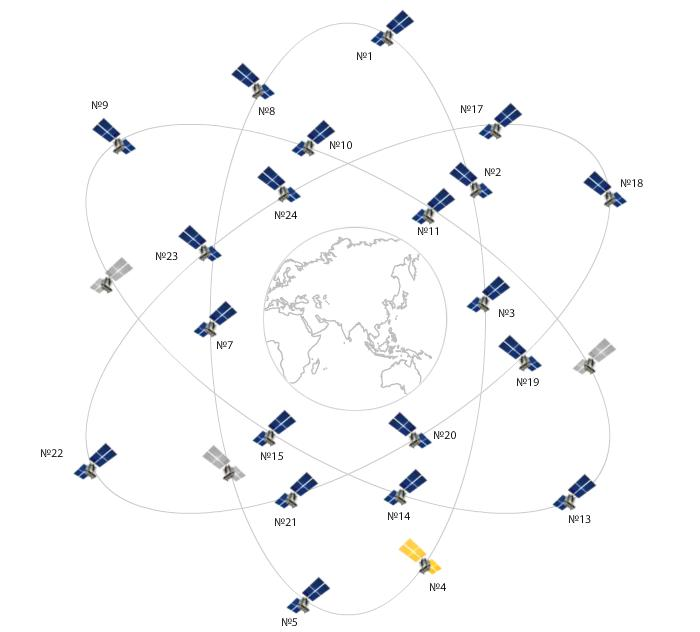
\includegraphics[scale=0.44]{GLONASS.jpg}
	\centering
	\caption{GLONASS constellatie \cite{LImgGLONASS}}
	\label{imgGLONASS}
\end{figure}

\subsubsection{GLONASS signalen}
Terwijl bij GPS de signalen mudolaties zijn van de draaggolven L1 en L2 voor alle satellieten, zijn bij GLONASS de frequenties van de draaggolf afhankelijk van het uitzendende kanaal. Er zijn 12 kanalen voor 24 satellieten \cite{LBibGPS3}. GLONASS maakt ook gebruik van de derde L5 frequentie. Deze wordt gebruikt door de GLONASS-K satellieten \cite{LBibGNSS9}.  
 
\subsection{Galileo}
\label{LGal}
Galileo is het Europees systeem \cite{LBibGNSS3, LBibGNSS4}. Het doel van Galileo is het aanbieden van een flexibelere en nauwkeurige positionerings service \cite{LBibGNSS4}. Bij de ontwikkeling van het systeem is gespecificeert dat het stand-alone bruikbaar moet zijn, maar dat het eveneens moet kunnen samen werken met andere diensten zoals GPS. Het moet goede positie- en tijds-diensten leveren \cite{LBibGalileo2}. De kostprijs wordt geschat tussen 2,2 en 2,9 miljard euro. De financiering komt van een gedeelde publieke en private vennootschap \cite{LBibGNSS8}. Galileo is ontworpen om Europa te voorzien van dezelfde GNSS capaciteit als dat van GPS \cite{LBibGNSS6}. De architectuur van Galileo specificeert een globaal integriteitsconcept. Dit wilt zeggen dat de nauwkeurigheid en de integriteit van de werking altijd wereldwijd bereikt moet worden en binnen de drempelwaarden moet blijven.  Het Galileo systeem voorziet verschillende gebruikersdiensten. E\'en van deze diensten is de Safety of Life service, dit is een groot voordeel van Galileo in vergelijking met GPS. In geval van een systeem fout moet de gebruiker binnen de zes seconden gewaarschuwd worden \cite{LBibGalileo}. Een uniek aspect van de satellieten die bij Galileo worden gebruikt is dat deze uitgerust zijn met een passieve waterstof maser. Dit zorgt voor een uitzonderlijke klok stabiliteit. Dit levert veel voordelen voor real-time navigatie, ppp en andere wetenschappelijke toepassingen \cite{LBibGNSS9}.

\subsubsection{Opbouw Galileo constellatie}
Tijdens het ontwikkelen van de opbouw van de constellatie is er geconcentreerd op twee opties. De eerste maakt gebruik van MEO satellieten. De andere maakt gebruik van een mengeling tussen MEO en GEO satellieten. De nadruk ligt op het leveren van hoge kwaliteit diensten. Dit met name in Europa en de noordelijke regio's. Omdat de constellatie gebruikt wordt voor commerci\"ele- en veiligheidstoepassingen, is het ontwikkeld om zeer robuust te zijn en toch economisch verantwoord. De constellatie die uiteindelijk gekozen is, is deze met de MEO satellieten \cite{LBibGalileo2}. De volledige constellatie zal bestaan uit 30 satellieten in drie orbitale vlakken. Het systeem is momenteel nog onder constructie \cite{LBibGNSS4}. De periode van een tocht om de aarde is 14 uur en 21 minuten. Er zijn 10 satellieten per vlak \cite{LBibGNSS6}. De straal van de baan is 23223 km. De satellieten zelf zijn van een gemiddelde grootte. Eens ze in hun baan zijn, wegen ze 650 kg en genereren een vermogen van 1500 Watt \cite{LBibGalileo2}. In de constellatie zijn eveneens vier In Orbit Validation (IOV) satellieten geplaatst \cite{LBibBeiDou3,LBibPPP2}.Deze satellieten ondersteunen testen en experimenten maar zijn nog niet goedgekeurd \cite{LBibGNSS9}. Figuur \ref{imgGalileo} toont een grafische weergave van de constellatie.

\begin{figure}[h!]
	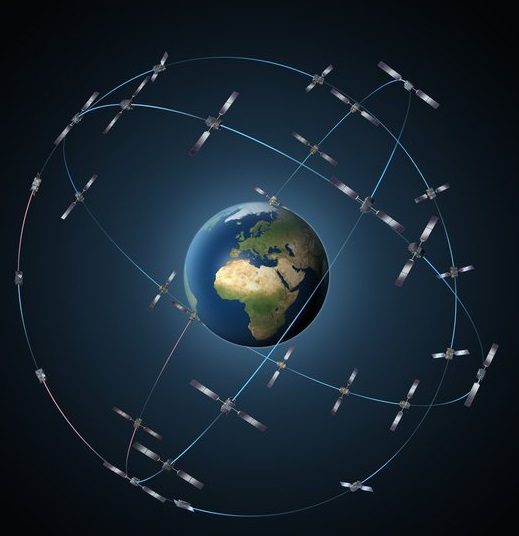
\includegraphics[scale=1.75]{Galileo.jpg}
	\centering
	\caption{Galileo constellatie \cite{LImgGalileo}}
	\label{imgGalileo}
\end{figure} 

\subsubsection{Galileo signalen}
Galileo zendt open signalen uit met een CP van 1575.42 MHz (E1), 1175.45 MHz (E5a), 1207.14 MHz (E5b) en 1195.795 MHz (E5a+b). Verder wordt voor commerci\"ele doeleinden een frequentie van 1278.75MHz (E6) gebruikt. Zoals uit de gegeven waarden afgeleid kan worden, delen Galileo en GPS de  L1/e1 en L5/E5a draaggolf \cite{LBibPPP2}. Doordat Galileo signalen beschikbaar stelt in verschillende frequentiebanden, kunnen lineaire combinaties van verschillende signalen gebruikt worden \cite{LBibGalileo3}. De toegang tot de E6 signalen is nog niet volledig gedefinieerd. Gebruikers kunnen vij toegang krijgen tot de signalen met geavanceerde multipad performantie in de E1 en E5a/E5b banden \cite{LBibGNSS9}. 

\subsection{BeiDou}
\label{LBeD}
BeiDou is het satelliet systeem binnen GNSS dat ontwikkeld is in China. Het systeem wordt vaak  aangeduid met de afkorting BDS \cite{LBibBeiDou}. De ontwikkeling van dit systeem volgt een drie stappen strategie. Dit zijn: demonstratie van het systeem, het regionale systeem en als laatste het globale systeem \cite{LBibBeiDou4}. Het voorziet PNT (Postioning, Navigation and Timing) services in de Aziatisch-Pacifische regio. Momenteel is BDS  beschikbaar voor regionale diensten. Hiervoor werd de werking in 2012 aangekondigd. De diensten leveren een goede nauwkerigheid aan zijn gebruikers \cite{LBibBeiDou, LBibGNSS9}. In 2020 zullen BDS signalen beschikbaar worden voor wereldwijde gebruikers. Ondertussen worden steeds meer stations uitgebreid met BDS ontvangers voor hoog-precisie GNSS toepassingen \cite{LBibBeiDou}.De nauwkeurigheid van DGNSS met BeiDou signalen is van hetzelfde niveau als dat van DGPS. BeiDou zorgt voor een goede geometrische dekking in de Aziatisch Pacifische regio. Het aantal zichtbare satellieten is groter dan zeven \cite{LBibBeiDou4}. 

\subsubsection{Opbouw constellatie}
De volledige constellatie telt 35 satellieten. Het zal volledig zijn tegen het einde van 2020 \cite{LBibGNSS4}. De constellatie van BeiDou is interessant omdat het verschilt van de andere reeds bestaande GNSS constellaties \cite{LBibBeiDou3}.  De constellatie bestaat momenteel uit 5 GEO satellieten, 5 IGSO satellieten verdeeld over 2 banen en 4 MEO satellieten in een baan met 27 878km als straal \cite{LBibBeiDou2}. De constellatie, opgebouwd uit die 14 satellieten, heeft zijn FOC bereikt in 2012 \cite{LBibBeiDou4}. De geometrie van de satellietbanen en hun dekking is symmetrisch ten op zichte van de evenaar \cite{LBibBeiDou5}.  De volgende stap in de ontwikkeling van de constellatie is het verder uitwerken van het MEO gedeelte \cite{LBibPPP2}. De opbouw van de constellatie wordt weergegeven in figuur \ref{imgBeiDou}.

\begin{figure}[hbp]
	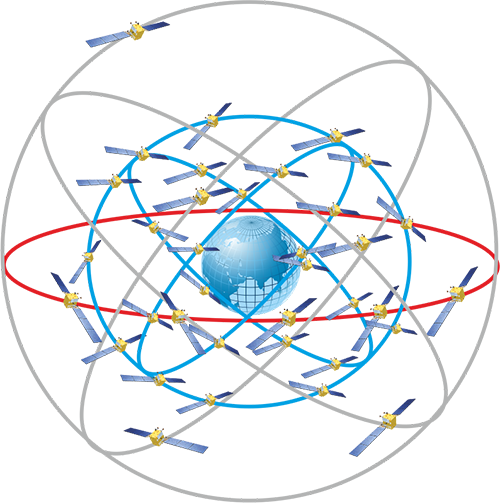
\includegraphics[scale=0.45]{BeiDou.png}
	\centering
	\caption{BeiDou constellatie \cite{LImgBeiDou}}
	\label{imgBeiDou}
\end{figure} 

\subsubsection{Signalen}
BeiDou stuurt signalen uit in drie frequenties: 1561.098 MHz (B1), 1207.14 Mhz (B2) en 1268.52 MHz (B3). Zoals afgeleid kan worden uit de gegeven waarden, delen Galileo een BeiDou de B2/E5b draaggolf \cite{LBibPPP2,LBibBeiDou4}. Deze drie signalen kunnen door een groot deel van multi-GNSS ontvangers ontvangen worden \cite{LBibGNSS9}. Het BeiDou systeem maakt gebruik van twee verschillende soorten navigatie berichten. Deze worden verzonden door de MEO/IGSO en GEO satellieten. Alle berichten zijn gebaseerd op 30-bit woorden en subframes met een lengte van 10 woorden \cite{LBibBeiDou5}.  

\subsection{Multi-GNSS}
Eens de vier systemen volledig ingezet zijn, zijn er meer dan 100 satellieten beschikbaar voor nauwkeurige PNT toepassingen. Door het opkomen van de twee nieuwere systemen (Galileo besproken in sectie \ref{LGal} en BeiDou besproken in sectie \ref{LBeD}) en het voortdurend moderniseren van GPS, besproken in sectie \ref{LGPS} en GLONASS, besproken in sectie \ref{LGLO} is de wereld van satelliet navigatie onderheving aan veranderingen \cite{LBibGNSS4}. Momenteel loopt er een Mutli-GNSS experiment (MGEX) dat data verzamelt van GPS, GLONASS, Galileo en BeiDou. De samenvoeging van multi-GNSS vergroot het aantal satellieten en bijgevolg wordt de geometrische observatie geoptimaliseerd \cite{LBibGNSS5}. 
MGEX dient als een kader voor het verhogen van het algehele bewustzijn van multi-GNSS binnen de wetenschappelijke- en ingenieursgemeenschappen. Eveneens gaan ze IGS deelnemers (centra die gebruik maken van GNSS data en lid zijn vna het IGS) vertrouwd maken met de nieuwe satelliet navigatie systemen. Als een minimum moeten alle MGEX stations GPS volgen en Galileo of BeiDou. GLONASS wordt door het grootste deel van de systemen gevolgd \cite{LBibGNSS9}.  De multiple-GNSS observaties met meerdere frequenties voorzien de onderzoekers van meerdere kansen om de aardse ionosferische variaties en gedragingen te onderzoeken. GNSS observaties kunnen gebruikt worden om ionosferische traagheids correcties en gerelateerd wetenschappelijk onderzoek \cite{LBibBeiDou}. Door het gemeenschappelijk gebruik van draaggolven tussen de verschillende systemen, is het gemakkelijker om de systemen samen te gebruiken \cite{LBibPPP2}. De aanwezigheid van multipad signalen resulteert in variaties en CP fouten \cite{LBibGalileo3}. 

\section{EUREF Permanent Netwerk}
\label{LEPN}
Het EUREF Permanent GNSS Network wordt ook wel EPN genoemd \cite{LBibEPN3,LBibEPN2,LBibEPN}. Het netwerk is gebaseerd op een relatie tussen site opperatoren van permanente GNSS sites, die bereid zijn om hun data met het publiek te delen. Het EPN werkt nauw samen met het IGS \cite{LBibEPN3}. Het netwerk is ontstaan in 1995 met ongeveer 30 permanente stations en vier analyse centra \cite{LBibEPN5}. Het EPN is momenteel opgebouwd uit 321 permanente GPS stations waarvan er ook GLONASS satellieten volgen. Alle EPN stations moeten L1 en L2 GPS signalen volgen, maar indien het mogelijk is, moeten ze ook het nieuwe L5 signaal volgen \cite{LBibEPN4}. Het grootste deel van de stations die opgenomen zijn in het EPN vormen eveneens een onderdeel van het IGS. Het primaire doel van EPN is het European Terrestrial Reference Systems (ETRS89) onderhouden. Dit gebeurt door de leden op vrijwillige basis \cite{LBibEPN, LBibEPN2}. Door de sterke groei van het EPN zijn er opportuniteiten onstaan om het netwerk te gebruiken buiten zijn initi\"ele doelen \cite{LBibEPN5}. Een doel van het netwerk is het beschikbaar stellen van GNSS data en precise co\"ordinaten van GNSS stations beschikbaar stellen aan het publiek. Nieuwe stations worden aan het netwerk toegevoegd zodra ze voldoen aan alle vereisten. Het EPN werkt met drie datacenters die gedefinieerd worden als regionale datacenters (RDC). Het Federal Agency for Cartography and Geodesy van Duitsland (BKG) en het Bundesamt fuer Eich- und Vermessungwensen Vienna(BEV)  datacenters, zijn verantwoordelijk voor de dagelijkse zaken. Alle EPN stations gaan op vooraf gedefinieerde wegen hun data op regelmatige basis doorsturen naar het BKG en het OLG \cite{LBibEPN2}. Het datacenter Royal Observatory of Belgium (ROB) doet dienst als datacenter van het centrale bureau van het EPN. Dit datacenter is verantwoordelijk voor het hosten van alle historische EPN RINEX data (Dit wordt verder besproken in sectie \ref{LRin}) met gecorrigeerde meta-data en 1 regionale broadcaster. \cite{LBibEPN2,LBibEPN3}. Het co\"ordineren van tijd analyse is eveneens een doel van het EPN. Dit om het EPN te versterken als geodetisch referentie netwerk. Van de nieuwe ge\"installeerde antennes is 90 procent een multi-GNSS antenne. Hiervan is 75 procent ontworpen om GNSS en GLONASS te obeserveren, 25 procent van de EPN antennes is bovendien ook klaar om Galileo te ontvangen. Het netwerk is dus continu onder constructie. \cite{LBibEPN3}. Een station kan officieel erkend worden als een EUREF station als \cite{LBibGNSS8}:
\begin{itemize}
	\item Het station ge\"installeerd is volgend de IGS standaard
	\item De log file van het station beschikbaar is op het EPN centraal bureau
	\item De data van het station beschikbaar is voor de EUREF gemeenschap
	\item De data van het station regelmatig geanalyseerd wordt door een van de EUREF analyse centra. 
\end{itemize} 
Om de installatie van EPN stations in dun bezette gebieden te promoten, is er een nieuwe regel in gebruik gesteld in verband met de locatie van het nieuwe station. Er moet een minimale afstand van 300 km zijn met een reeds bestaand EPN station. Een mogelijke uitzondering op deze regel is dat als het station in staat is om uurlijks data te leveren en bijdraagt tot het EPN Special Projects, het wel mag toetreden. Dankzij deze nieuwe regel, sturen 45 \% van de stations uurlijks data \cite{LBibEPN6}. Binnen het EPN wordt de overschakeling naar een nieuwe set van antenne calibraties simultaan met het IGS gemaakt. Het grootste verschil met het IGS is dat binnen het EPN de individuele ontvanger antenne callibraties online beschikbaar zijn \cite{LBibEPN4}.

\subsection{Management en Co\"ordinatie}
De activiteiten binnen het EPN worden sinds het ontstaan van het EPN in 1998 geco\"ordineerd en gestuurd door het EUREF Technical Working Group (EUREF TWG). Nu wordt dit gedaan door het EUREF Governing Board.  Een netwerk co\"ordinator zorgde voor het dagelijks management van het netwerk. Door de groei van het netwerk en ook het takenpakket, heeft  een reorganisatie plaatsgevonden. Er zijn momenteel drie eenheden die instaan voor de co\"ordinatie van het netwerk. Namelijk de EPN coordination groep, het EPN central bureau en de EPN special projects \cite{LBibEPN6}. 
De EPN coordination group is als volgt samen gesteld \cite{LBibEPN8}:
\begin{description}
	\item[Netwerk Co\"ordinator] Carine Bruyninx, Royal Observatory of Belgium
	\item[Analyse Co\"ordinator] Tomek Liwosz, Warsaw University of Technology and Military University of Technology
	\item[Referentieframe Co\"ordinator] Juliette Legrand, Royal Observatory of Belgium
	\item[Troposfeer Co\"ordinator] Rosa Pacione, Italian Space Agency
\end{description}

\section{Communicatie}
\label{LCom}
Er zijn verschillende manieren om GNSS data uit te wisselen. Hier gaat in het practische gedeelte van de masterproef aan gewerkt wordt.  Een manier om GNSS data uit te wisselen is RINEX, deze wordt besproken in sectie \ref{LRin}. Dit data formaat is niet beschikbaar voor real-time data transmissie. Om wel aan real-time transmissie te kunnen doen moeten er drie componenten aanwezig zijn. Het eerste is het transmissie protocol dat instaat voor de levering van de data over een netwerk en dat eveneens controle mechanismen voorziet. Het data formaat is de tweede component, dit is een overeenkomst om de uitgezonden bit sequentie te kunnen vertalen naar zinvolle informatie. De laatste component is de data communicatie link die instaat voor de manier waarop data van de ene naar de andere partij getransporteerd wordt. Er zijn twee standaard protocols om GNSS data over het internet te verdelen. Het eerste is RTCM, dit wordt verder besproken in sectie \ref{LRTC}. De tweede mogelijkheid is Real-Time IGS (RTIGS) \cite{LBibRTCM} en wordt verder niet besproken in deze literatuurstudie. Dit omdat het tijdens het verder verloop van de masterproef niet behandeld wordt. Standaardisatie van dataformaten is een belangrijk aspect voor management, analyse en uitwisseling van GNSS data \cite{LBibRINEX}. De modernistatie van de constellaties zorgt voor verscheidene nieuwe signalen en toepassingen. Deze nieuwe signalen vormen een uitdaging en hebben een impact op verscheidene toepassingen. Hieronder volgt de manier waarop ze doorgestuurd worden \cite{LBibRINEX2}. 

\subsection{RINEX dataformaat}
\label{LRin}
RINEX is een afkorting voor Reciever INdependant EXchange. Het is reeds in gebruik sinds het begin van GPS toepassingen. Het wisselt GPS data uit in een ASCII bestandsformaat voor wetenschappelijke en geodetische toepassingen \cite{LBibRTCM}. Dit garandeert een gemakkelijke uitwisseling tussen verschillende computersystemen, maar het gebruik van RINEX data bestanden is niet zo eenvoudig aangezien het geavanceerde algortimen en computercodes nodig heeft. Deze zijn meestal gepatenteerd of enkel beschikbaar voor de personen die deel uit maken van een internationaal netwerk van GPS ontvangers \cite{LBibGPS5}. RINEX is een internationale standaard. Typisch worden uurlijkse of dagelijkse data gearchiveerd in het RINEX bestandsformaat en wordt de data beschikbaar door een FTP server om te downloaden. Er zijn verschillende toepassingen die een post-processing methode gebruiken. RINEX is strikt bestand gebaseerd en is niet beschikbaar voor real-time data transmissie \cite{LBibRTCM}. Dit formaat is oorspronkelijk ontworpen voor de data van GPS. Later is dit uitgebreid naar GLONASS zonder de basis structuur van het formaat aan te passen \cite{LBibRINEX}. De RINEX data afkomstig van GPS ontvangers bevat hoofdzakelijk \cite{LBibGPS5}:
\begin{itemize}
	\item C1: C/A code pseudo range in meters op L1 frequentie
	\item P2: P code pseudo range in meters op L2 frequentie
	\item L1: L1 CP in cycles op L1 frequentie
	\item L2: L2 CP in cycles op L2 frequentie
\end{itemize}
 Er zijn momenteel drie verschillende RINEX versies. Namelijk versie 1, 2 en 3.00. RINEX versie  2 wordt veel gebruikt in de geodetische gemeenschap, ook door het IGS. RINEX versie 2 is niet in staat om alle huidig beschikbare datatypes afkomstig van L2 ontvangers te ondersteunen. Een grote herziening van het RINEX formaat levert versie 3.00. Men verwacht dat versie 3.00 de nieuwe standaard versie van het IGS zal worden. Een groot nadeel van het RINEX formaat is dat de bestandsgrootte van de observatie bestanden groot worden. Hierdoor zijn er compacte RINEX formaat versies gemaakt. Deze worden aangeduid met de namen 1.0 en 3.0. Compact RINEX formaat 1.0 is een compressie formaat dat compatiebel is met RINEX versie 2. Het compacte RINEX 3.0 formaat is compatiebel met RINEX 3.00. Naar verwachtingen is RINEX 3.00 compatiebel met alle nieuwe niet gecomprimeerde versies van RINEX zolang de structuur van de RINEX bestanden ongewijzigd blijft.  De compacte RINEX formaten zijn compatiebel met RINEX observatie data bestanden, niet voor navigatie berichten of meterologische data bestanden \cite{LBibRINEX}. De laatste versie van RINEX is 3.03. De opbouw van een RINEX bestand wordt weergegeven in tabel \ref{TabRINEX}.
 
 %
 \newcommand*{\MyIndent}{\hspace*{0.5cm}}%
 \begin{table}[hbp]
 	\caption{Vereenvoudigde samenstelling van een RINEX bestand}
 	\centering		
 	\begin{tabular}{|p {10cm}|}	
 		\hline
 		RINEX hoofding \\
 		... \\ \hline
 		epoch hoofding\\ \hline
 		\MyIndent observaties satelliet i \\ \hline
 		\MyIndent observaties satelliet j \\ \hline
 		... andere satellieten ... \\ \hline
 		epoch hoofding\\ \hline
 		\MyIndent observaties satelliet i \\ \hline
 		\MyIndent observaties satelliet j \\ \hline
 		... andere satellieten ... \\ \hline
 		... andere epochs ... \\ \hline	
 	\end{tabular}
 	\label{TabRINEX}
 \end{table}
 
 
\subsubsection{Strategi\"en voor kwaliteitscontrole}
Er zijn verscheidene manieren om na te gaan of een RINEX bestand voldoet aan een aantal vereisten. Het eerste is een filter. Er wordt nagegaan of het bestand de nodige onderdelen bevat. Zo wordt bijvoorbeeld getest of de RINEX hoofding aanwezig is en de nodige lijnen bevat. Eveneens wordt getest of het geen corrupt bestand is. Een volgende methode is om de bestanden te gaan vergelijken met een IGS nauwkeurige bron. Het nadeel hiervan is dat er zo een bron beschikbaar moet zijn \cite{LBibRINEX3}. 

\subsection{RTCM dataformaat}
\label{LRTC}
RTCM staat voor Radio Technical Commission for Maritime Services \cite{LBibGLONASS}. De sterke vraag voor real-time DPGS heeft geleid tot de oprichting van het Special Comite 104 (afgekort tot SC104) \cite{LBibRTCM}. RTCM is het standaard formaat gebruikt voor RTK en DPGS correctie data. Het is momenteel het formaat dat het meest gebruikt wordt \cite{LBibRTK3}. Momenteel zijn meerdere internationale standaarden voor RTCM \cite{LBibRTCM}, deze worden verder besproken. RTCM data wordt verzonden als een continue binaire datastroom. Typisch wordt een volledig RTCM data record verstuurd binnen een seconde. RTCM comprimeert de verschillende onderdelen van een record in verschillende berichttypes. Een overzicht hiervan is te zien in tabel \ref{TabRTCMBer} \cite{LBibRTCM3}.

\begin{table}[hbp]
	\caption{RTCM record, verdeeld in verschillende berichttypes}	
	\centering	
	\begin{tabular}{|p {5cm}|}	
		\hline
		Bericht 1 \\ \hline
		Bericht 2 \\ \hline
		... \\ \hline
		Bericht n \\ \hline
	\end{tabular}
	\label{TabRTCMBer}
\end{table}

Elk bericht binnen een data record bevat een hoofding en een berichtinhoud. Dit wordt verduidelijkt in tabel \ref{TabRTCM2} \cite{LBibRTCM3}.

\begin{table}[hbp]
	\caption{RTCM bericht, verdeeld in hoofding en bericht}	
	\centering	
	\begin{tabular}{|p {5cm}|}	
		\hline
		Bericht - Hoofding \\ \hline
		Bericht - Inhoud \\ \hline
	\end{tabular}
	\label{TabRTCM2}
\end{table}

Het berichttype, de tijdsinformatie, de ID van het referentiestation, de lengte van het bericht en andere informatie zoals monitoring status zitten omvat in de hoofding. De inhoud bevat de relevante werkingsdata voor elk data type. De lengte van het bericht is afhankelijk van het data type. De hoofding en de inhoud worden beschermd door pariteitbits. Zo kunnen fouten relatief gemakkelijk gedetecteerd worden. Een RTCM data record hoeft niet alle berichttypes te bevatten. Sommige berichten moeten elke seconde verstuurd worden. Andere worden automatisch verzonden op een gewenst interval. Als een datarecord korter is dan het zendinterval, zal geen andere data verzonden worden in de reserende tijd. Omdat de data real-time verzonden wordt, moet er bij een fout in het record gewacht worden op het volgende record. Er is geen tijd om het onjuiste record nog een keer te verzenden \cite{LBibRTCM3}. 

\subsubsection{RTCM - 2.0}
RTCM versie 2.0 is belangrijk voor DPGS toepassingen. Het wordt gebruikt sinds 1990. Het bevat alle nodige informatie om correctie data en andere informatie te sturen voor DPGS toepassingen. Er zijn nieuwe berichttypes speciaal voorzien voor DPGS toepassingen. Deze worden weergegven in tabel \ref{TabRTCM2.0} \cite{LBibRTCM3}.

\begin{table}[hbp]
	\caption{RTCM-2.0 berichttypes relevant voor DGPS}		
	\centering
	\begin{tabular}{|c|p {8cm}|p {6cm}|}	
		\hline
		Type & Inhoud & Frequentie \\ \hline
		1 & Differenti\"ele correcties voor code observaties & In elk record, typisch elke seconde \\ \hline
		2 & Delta correcties & Automatisch bij elke verandering in satellietbaan, voor elke uursverandering \\ \hline
		3 & Co\"ordinaten van het referentiestation & Indien nodig, typisch in intervallen van een minuut \\ \hline
		16 & Elke gewenste alfanumerische tekst (bv de naam en telefoonnummer van het referentie station) & Indien nodig \\ \hline
		59 & Gebruiker gedefinieerd berichttype & Indien nodig \\ \hline
	\end{tabular}
	\label{TabRTCM2.0}
\end{table}
De DPGS nauwkeurigheid die je kan bereiken met RTCM 2.0 bedraagt 1 meter. Er zijn ook nog andere nieuwe berichttypes in vergelijking met de eerste versie van RTCM. Deze versie bevat geen CP informatie dus geen RTK toepassingen zijn mogelijk. Een volledig RTCM 2.0 record bevat ongeveer 1200 bits \cite{LBibRTCM3}. 

\subsubsection{RTCM - 2.1}
Deze versie is in gebruik sinds 1993. De volledige inhoud van RTCM 2.0 blijft behouden bij deze versie \cite{LBibRTCM3}. RTCM versie 2.1 bevat vier berichttypes die specifiek voor RTK data transmissie zijn. Berichttype 18 en 19 bevatten ruwe informatie over de CP en berichttypes 20 en 21 zijn voorzien voor de transmissie van de CP en de pseudorange correcties \cite{LBibDGPS}. Een beperking is de nodige snelheid waarmee de data verzonden moet worden om de CP correcties van het basisstation naar het mobiele station te brengen. Bij RTCM 2.1 is een dataframe van meer dan 4800 bits nodig voor alle zichtbare satellieten. De meeste toepassingen willen elke seconde een update. Dit zorgt ervoor dat er een zeer hoge frequentie nodig is om alle informatie te verzenden \cite{LBibRTCM4}.

\subsubsection{RTCM - 2.2}
Versie 2.2 is de nieuwe standaard sinds 1998. In vergelijking met versie 2.1 omvat deze versie een paar uitbereidingen, zodat data afkomstig van GLONASS satellieten ook verwerkt en opgeslagen kan worden. Differenti\"ele GLONASS correcties worden opgeslagen in berichttype 31. Dit is op dezelfde manier opgebouwd als berichttype 1 voor DGPS data. Omdat berichttypes 18 tot 21 nu ook GLONASS data moeten kunnen verwerken, zijn ze niet langer compatibel met versie 2.1. 

\subsubsection{RTCM - 2.3}
RTCM versie 2.3 is voor het eerst gepubliceerd in 2001.  Voor geodetische toepassingen zijn de definities van antennetypes en antenne referentiepunten interessant. Berichttypen 18 tot en met 21 zijn compatibel met versie 2.2 \cite{LBibRTCM3}. 

\subsubsection{RTCM - 3.0}
Er is een update gebeurd naar versie 3.0. Deze versie is ontwikkeld om RTK operaties te verbeteren en netwerk RTK te ondersteunen. Alle RTCM 3.0 berichten beginnen met een 8-bit vaste sequentie, dit is de preamble. Deze wordt gevolgd door 6 gereserveerde bits. Elke berichtlengte is variabel en is afhankelijk van het berichttype. Een overzicht van de structuur van een RTCM versie 3 bericht is terug te vinden in tabel \ref{TabRTCM}.

\begin{table}[hbp]
	\caption{RTCM versie 3 frame structuur}	
	\centering	
	\begin{tabular}{|c|c|c|c|c|}	
		\hline
		Preamble & Gereserveerd & Bericht lengte & Variabele lengte data bericht & CRC \\ \hline
		8 bits & 6 bits & 10 bits & Variabele lengte, geheel aantal bytes & 24 bits \\ \hline
	\end{tabular}
	\label{TabRTCM}
\end{table}

RTCM versie 3.0 is momenteel het meest populaire formaat \cite{LBibRTCM}. De grootte van de berichten en de verpakkingsoverhead maakt dat dit formaat voor vele commerci\"ele toepassingen niet effeci\"ent genoeg is \cite{LBibDGPS}.  

\subsubsection{RTCM - 3.1}
De aanpassingen de gemaakt zijn ten op zichte van versie 3.0 hebben te maken met gegevens in verbant met de satellietbanen. Verder beschikt 3.1 ook over een betere bericht beschrijving. Er is eveneens een mogelijkheid om PPP gegevens te verzenden via RTCM - 3.1.

\subsubsection {RTCM - 3.2}
Met RTCP versie 3.2 is het mogelijk om gegevens in verband met satellietbanen van Galileo te versturen. 

\subsubsection{RTCM - 3.3}
Met de laatste versie van RTCM kunnen gegevens over de BeiDou constellatie verzonden worden. 

\subsubsection{RTCM++}
Het RTCM++ formaat is ontwikkeld in 1993. Dit om de tekorten van RTCM versie 2.1 op te vangen, voornamelijk de nauwkeurigheid en het volume van de verzonden data. Aangezien de inhoud van RTCM++ data indentiek is aan RTCM 2.1 correctie data, is minimaal de zelfde nauwkeurigheid van 1 cm haalbaar \cite{LBibRTCM3}. RTCM++ is een compact dataformaat voor de CP correcties. De complete dataset voor alle zichtbare satellieten bedraagt maximaal 2400 bits, dit in vergelijking met de 4800 bits bij RTCM 2.1 een betere optie omdat de frequentie waarmee de data moet worden verzonden niet zo hoog moet zijn \cite{LBibRTCM4}. RTCM++ wordt niet gebruikt. 

\subsection{NTRIP}
\label{LNTR}
Networked Transport of RTCM via Internet Protocol of kortweg NTRIP \cite{LBibNTRIP,LBibNTRIP3}. NTTRIP is een protocol ontwikkeld in 2004 \cite{LBibNTRIP3} als een project onder EUREF \cite{LBibNTRIP4}. Men maakt gebruik van het internet om de realtime GNSS data uit te wisselen en te verzamelen. NTRIP is een HTTP(Hypertext Transfer Protocol) stateless applicatie level protocol om GNSS te streamen over het internet \cite{LBibNTRIP}. NTRIP is de interface die gebruikt wordt voor MGEX toepassingen \cite{LBibGNSS9}. De toepassing die men in gedachte had bij het ontwerpen van het protocol is het doorsturen van RTCM data, maar het protocol kan gebruikt worden om GNSS data in eender welk formaat door te sturen. De enige beperking is een maximum snelheid van 10 kb/s en een minimum van 100b/s \cite{LBibNTRIP3}.  Het doel is om real-time data uit te wisselen, maar ook om afgeleide producten te broadcasten, voornamelijk DGPS \cite{LBibNTRIP2}. De nodige brandbreedte hiervoor is niet groot in vergelijking met bijvoorbeeld Internet Radio \cite{LBibNTRIP}. Hierdoor wordt de NTRIP techniek een alternatief voor het verzenden van DGPS data tegenover andere  wereldwijde broadcasting technieken. Het internet is uitermate goed geschikt om data door te sturen tussen verschillende providers over een grote afstand \cite{LBibNTRIP2}. Het is gebaseerd op software die oorspronkelijk bedoeld was voor MP3-formaten. Dit blijk wel aangepast te zijn voor GNSS stromen met data snelheden tussen 0.5 en 5 kbit/s. \cite{LBibGPS}. Een ander voordeel is dat tegenwoordig op veel plaatsen internet verbinding voorzien is \cite{LBibNTRIP}. Verder is er ook geen vermindering van de positie voorstelling door gebruik te maken van NTRIP. Een ander groot voordeel is dat datastromen van referentie stations simultaan beschikbaar worden via \'e\'en communicatie techniek. Men moet er wel rekening mee houden dat de nodige servers moeten verbonden worden aan het internet via intergeconnecteerde broadcasters met een voldoende grote bandbreedte.  De generatie van DPGS correctie data wordt meestal direct op de GPS ontvanger gedaan, maar hij kan eveneens bepaald worden van observaties die verkregen worden door verschillende referentie stations in het netwerk. De datastroom wordt dan doorgegeven aan een server die de datastroom vervolgens beschikbaar stelt over het internet via een geschikt protocol \cite{LBibNTRIP2}. Het gevolgde pad van de data wordt weergegeven in figuur \ref{imgNTRIP2}.

\begin{figure}[hbp]
	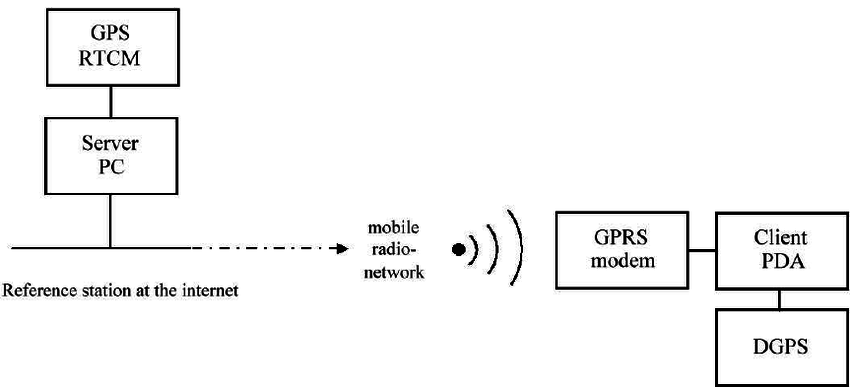
\includegraphics[scale=0.4]{NTRIP2.png}
	\centering
	\caption{RTCM data stroom op het internet \cite{LBibNTRIP2}}
	\label{imgNTRIP2}
\end{figure} 

\subsubsection{Communicatie}
Figuur \ref{imgNTRIPCom} toont hoe NTRIP communicatie werkt. De gebruiker, dit is de NTRIPClient ontvangt de correctie data van het controle centrum via het internet. De data wordt in NTRIP formaat over het internet verzonden. De communicatie tussen het controle center (NTRIPCaster) en het referentiestaion (NTRIPServer) gebeuren via NTRIP. Zowel gebruikers als referentiestations ontvangen satelliet data. De correctievoorziening is verantwoordelijk voor de NTRIPCaster in het controle centrum \cite{LBibNTRIP4}. De afstand tussen het referentie station en de client met het verbonden station is opgedeeld in twee delen. Het grootste deel van de afstand bestaat uit een bedrade internet verbinding. Het overige deel wordt overbrugd door mobiele telefonie technologie \cite{LBibNTRIP2}.

\begin{figure}[h!]
	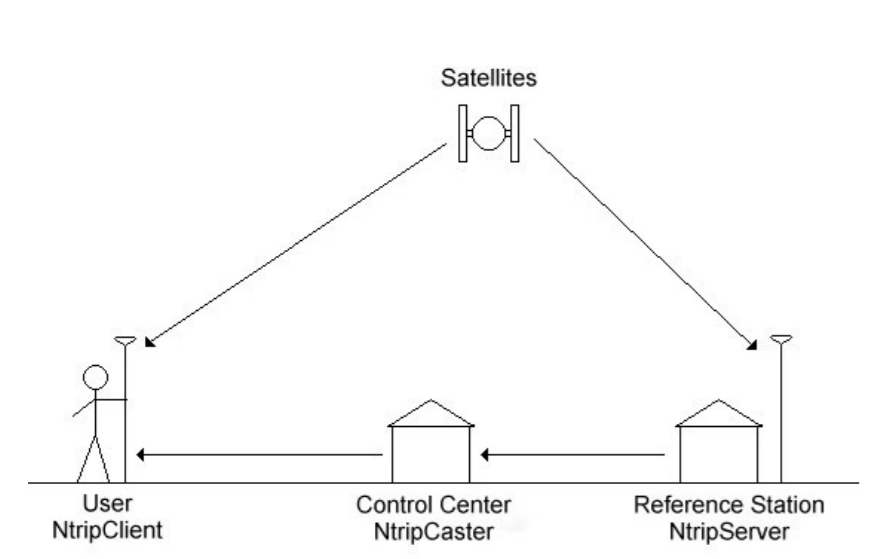
\includegraphics[scale=0.55]{NTRIPCommunication.png}
	\centering
	\caption{Schematisch overzicht NTRIP communicatie \cite{LBibNTRIP4}}
	\label{imgNTRIPCom}
\end{figure}

\subsubsection{Opbouw van NTRIP software}
\label{LONS}
NTRIP wordt ge\"implemeneteerd in vier grote componenten. Namelijk NTRIPSources, NTRIPClients, NTRIPServers en NTRIPCasters. De NTRIPCaster is het HTTP server programma terwijl NTRIPClients en NTRIPServers reageren zoals HTTP clients\cite{LBibNTRIP}.  In figuur \ref{imgNTRIP} staat een overzicht van de opbouw van het NTRIP streaming systeem.

\begin{figure}[hbp]
	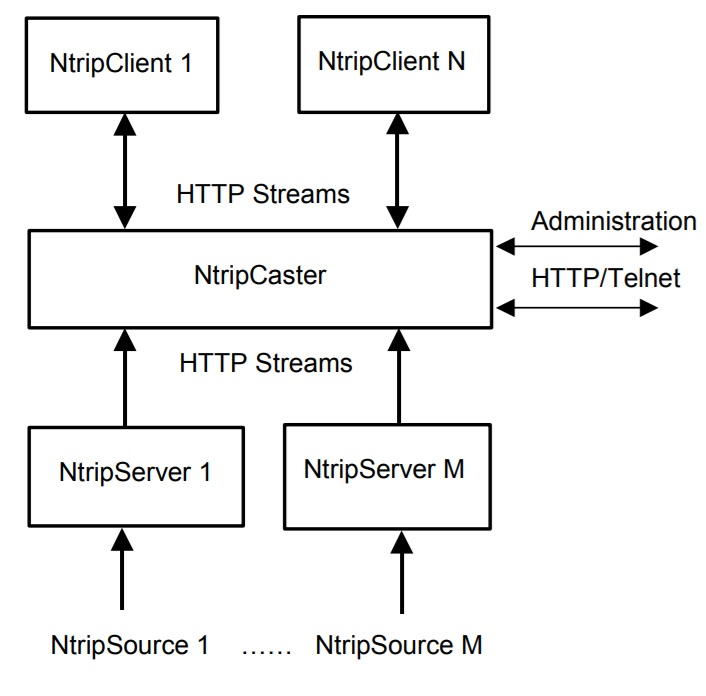
\includegraphics[scale=0.55]{NTRIP.jpg}
	\centering
	\caption{NTRIP streaming systeem \cite{LBibNTRIP}}
	\label{imgNTRIP}
\end{figure} 
NTRIP is gebaseerd op een subset van het vaak gebruikte HTTP en is bijgevolg gebaseerd op TCP. Daaruit volgt dat het streamen gebeurt vanuit een enkele IP Poort. Meestal is dit poort 80 of 2101 \cite{LBibNTRIP3}. 

\paragraph{NTRIPCaster}
 NTRIPCasters gaan de administratie tussen clients en servers afhandelen \cite{LBibGPS}. NTRIPCaster is een stream-splitser- en broadcaster- component. Momenteel zijn er acht NTRIPCasters in Europa \cite{LBibNTRIP}. De NTRIPCasters gaan, zoals vaak gebeurt bij internet radio implementaties de binnenkomende datastromen dupliceren, zodat hij door meerdere gebuikers simultaan ontvangen kan worden \cite{LBibNTRIP2}. NTRIP omvat de voorziening van metadata door een Source Table die onderhouden wordt door de NTRIPCaster \cite{LBibNTRIP3}. Deze tabel bevat informatie over de NTRIPSources maar ook over de netwerken van sources en andere broadcasters. Elke NTRIPSource wordt ge\"identificeerd door een uniek aanhechtingspunt. Alle verzonden berichten met NTRIP worden ofwel ontvangen door de NTRIPCaster of verzonden door de NTRIPCaster \cite{LBibNTRIP4}. EUREF bevat 3 NTRIPCasters. Hiervan staat er \'e\'en in ROB. 
 
\paragraph{NTRIPSource}
De NTRIPSources stellen de bronnen van de GNSS data voor. Deze worden gevoed aan het systeem. Een  NTRIPSource kan een GNSS ontvanger zijn die obeservaties verstuurd. Een andere mogelijk heid is dat het een NGSs ontvanger is de DGPS correctie data gaat verzenden \cite{LBibNTRIP3}. NTRIPSource is een geografisch stationair punt dat een conutinue RTCM datastroom levert. De data wordt dan verzonden naar de NTRIPServer die de verdere transfer naar de NTRIPClient zal regelen \cite{LBibNTRIP4}.

\paragraph{NTRIPServer}
NTRIPServers gaan datastromen vervoeren \cite{LBibGPS}. NTRIPServers ontvangt RTCM data van een NTRIPSource en gaat dit doorsturen naar een NTRIPCaster in NTRIP formaat. Om een NTRIPServer te installeren moet je het mountpunt en het wachtwoord kennen \cite{LBibNTRIP4}.
 
\paragraph{NTRIPClient}
NTRIPClients gaan data ontvangen van de gewenste bronnen via de NTRIPCaster \cite{LBibNTRIP}. De NTRIPClient is de component die ge\"installeerd is in het toestel van de gebruiker dat GPS gaat ontvangen. Voor sommige technieken, zoals bij Virtueel Reference Station, moet de NTRIPClient in staat zijn om zijn positie door te sturen naar de NTRIPCaster. Deze mogelijkheid wordt bij NTRIP ondersteunt \cite{LBibNTRIP4}.



